% Software Requirements Specification
% TeX-master: ../report.tex  (graphicspath is images/)

\section{Introduction}

\subsection{Purpose}
This document defines the requirements for the \textbf{BookForMe} platform. The purpose of BookForMe is to address inefficiencies and fragmentation in booking informal, local services (such as sports courts, salons, and gaming zones) within Karachi. The system replaces unstructured communication and manual record-keeping with a centralized, intelligent, and reliable platform.

It provides a streamlined booking interface for end-users alongside a social community layer for players. Vendors receive tools to manage bookings and availability across all channels, including an autonomous AI assistant on WhatsApp, reducing operational friction and revenue loss from missed or mishandled requests.

\subsection{Scope}
The BookForMe system comprises four primary components operating together:
\begin{enumerate}
  \item \textbf{User-facing mobile application:} A React Native (Expo) app through which customers discover venues, view real-time slot availability, place bookings, and participate in social features including friends, direct messaging, forums, matchmaking, and a ranked leaderboard.
  \item \textbf{Vendor dashboard:} A vendor-facing React Native interface to register, manage a business profile (services, pricing, operating hours), view a consolidated booking calendar with live slot status, approve or reject pending payments, and connect a WhatsApp Business account.
  \item \textbf{AI agent backend:} The intelligent engine built in Python (FastAPI and LangGraph). It receives WhatsApp traffic via webhooks, performs bilingual (Roman Urdu/English) natural language understanding using Groq (Qwen 3 32B), manages stateful conversational booking workflows, enforces concurrency control via Firestore transactions, and coordinates payment proof and vendor approval flows.
  \item \textbf{Admin control panel:} A platform-level administrative interface for platform governance: vendor registration approval and moderation, slot generation, stale lock release, and oversight of pending payments across all vendors.
\end{enumerate}

\section{Functional Requirements}

\subsection{Module: User (Booking \& Discovery)}
\begin{itemize}
  \item \texttt{FR-CUST-01}: The system shall allow users to browse and search registered vendors by service category (e.g., Padel, Futsal, Cricket) and location area.
  \item \texttt{FR-CUST-02}: The system shall provide filtering options (e.g., price, area, sport type).
  \item \texttt{FR-CUST-03}: The system shall display vendor profiles including name, location, services offered, and pricing.
  \item \texttt{FR-CUST-04}: The system shall present a real-time live court grid showing available, held, and booked slots per court per time block.
  \item \texttt{FR-CUST-05}: The system shall allow users to select an available time slot and confirm a booking.
  \item \texttt{FR-CUST-06}: The system shall confirm successful bookings to the user via the app interface.
\end{itemize}

\subsection{Module: User (AI Chat \& Discovery)}
\begin{itemize}
  \item \texttt{FR-CUST-07} (Smart filter): The system shall provide an in-app AI chat interface that parses natural-language queries in English or Roman Urdu (e.g., ``Aaj Raat DHA mei konsa padel available hei under 2000'') and returns filtered venue results with available slots.
  \item \texttt{FR-CUST-08}: The in-app AI assistant shall return matching venues, available slot times, and pricing in a single response.
\end{itemize}

\subsection{Module: User (Social \& Community)}
\begin{itemize}
  \item \texttt{FR-SOC-01}: The system shall provide user registration and login with role selection (Customer or Vendor).
  \item \texttt{FR-SOC-02}: The system shall allow users to create and manage a public profile.
  \item \texttt{FR-SOC-03}: The system shall provide a friend system: send, accept, and deny friend requests.
  \item \texttt{FR-SOC-04}: The system shall allow users to send and receive private direct messages with friends.
  \item \texttt{FR-SOC-05}: The system shall provide a community forum where users can create, view, like, and comment on public posts.
\end{itemize}

\subsection{Module: User (Matchmaking \& Ranking)}
\begin{itemize}
  \item \texttt{FR-MATCH-01}: The system shall allow users to create and join open matches (Casual or Ranked) for sports such as Padel, Futsal, and Cricket.
  \item \texttt{FR-MATCH-02}: The system shall calculate and update user Elo ratings based on ranked match outcomes.
  \item \texttt{FR-MATCH-03}: The system shall display a public leaderboard of top-ranked players, filterable by sport, showing rank, points, and tier (e.g., Silver).
\end{itemize}

\subsection{Module: Vendor}
\begin{itemize}
  \item \texttt{FR-VEND-01}: The system shall provide secure registration and login for vendors, subject to admin approval before activation.
  \item \texttt{FR-VEND-02}: Vendors shall be able to create and manage their business profile (services, pricing, operating hours).
  \item \texttt{FR-VEND-03}: Vendors shall be able to view a live court grid calendar showing all bookings by court, time, and booking source (WhatsApp or walk-in).
  \item \texttt{FR-VEND-04}: The vendor dashboard shall display daily revenue, bookings count, pending action items, and upcoming unbooked slots.
  \item \texttt{FR-VEND-05}: The system shall provide an interface for vendors to generate availability slots and manage bookings.
  \item \texttt{FR-VEND-06}: The vendor dashboard shall provide an interface to review and approve or reject pending payments.
  \item \texttt{FR-VEND-07}: The system shall allow vendors to connect their WhatsApp Business account to activate the AI receptionist.
\end{itemize}

\subsection{Module: AI Agent (WhatsApp Receptionist)}
\begin{itemize}
  \item \texttt{FR-AGENT-01}: The system shall receive inbound WhatsApp messages via a configured Meta webhook.
  \item \texttt{FR-AGENT-02}: The system shall send outbound WhatsApp replies (slot listings, confirmations, rejections) via the WhatsApp Business API.
  \item \texttt{FR-AGENT-03}: The system shall process inbound messages in English and Roman Urdu to extract booking intent and entities (service, date, time, area).
  \item \texttt{FR-AGENT-04}: The system shall maintain full conversational context (dialogue state) for ongoing WhatsApp interactions, persisted in Firestore across delays.
  \item \texttt{FR-AGENT-05}: Based on NLU output and real-time availability, the system shall present matching slots to the user and accept confirmation.
  \item \texttt{FR-AGENT-06}: The system shall implement Optimistic Concurrency Control via Firestore transactions to prevent double-booking across all channels simultaneously.
  \item \texttt{FR-AGENT-07}: After a user confirms a booking, the system shall request payment proof (screenshot) and set the booking to a hold state with an expiry window.
  \item \texttt{FR-AGENT-08}: Upon receiving the screenshot, the system shall update the booking to pending approval, attach the image, and notify the vendor dashboard.
  \item \texttt{FR-AGENT-09}: Upon vendor approval, the system shall update the booking status to confirmed and send a confirmation message with a booking reference to the user on WhatsApp.
\end{itemize}

\subsection{Module: Admin}
\begin{itemize}
  \item \texttt{FR-ADMIN-01}: The system shall provide a platform administrator interface displaying pending vendors, pending payments, locked slots, and total active vendors.
  \item \texttt{FR-ADMIN-02}: The system shall allow admins to approve, suspend, or delete vendor accounts.
  \item \texttt{FR-ADMIN-03}: The system shall allow admins to generate availability slots across all vendors for a configurable window (e.g., next 14 days).
  \item \texttt{FR-ADMIN-04}: The system shall allow admins to release stale slot locks caused by abandoned booking sessions.
\end{itemize}

\subsection{Use Case Diagrams}
\label{sec:srs-usecases}

Figure~\ref{fig:srs-block} shows the high-level system overview. The use case interactions are summarized below:

\begin{itemize}
  \item \textbf{Customer} uses the mobile app to log in, discover venues, book slots, use the AI chat filter, and access social features (forum, friends, matches, leaderboard).
  \item \textbf{WhatsApp user} interacts with the AI receptionist: sends booking requests in English/Roman Urdu, confirms a slot, submits payment proof, and receives a confirmation.
  \item \textbf{Vendor} uses the vendor dashboard to manage their profile, view the live court calendar, handle payment approvals, and link their WhatsApp account.
  \item \textbf{Admin} uses the admin panel to approve vendors, manage slots, and oversee payments.
\end{itemize}

\section{Non-Functional Requirements}

\subsection{Performance}
\begin{itemize}
  \item \texttt{NFR-PERF-01}: Key app screens (vendor search, live court grid) shall load within 30 seconds on a stable mobile connection.
  \item \texttt{NFR-PERF-02}: The AI agent NLU processing for a WhatsApp message shall complete within 60 seconds.
  \item \texttt{NFR-PERF-03}: Total time from receiving a WhatsApp availability query to sending the initial response shall not exceed 60 seconds.
  \item \texttt{NFR-PERF-04}: The WhatsApp webhook shall handle at least four simultaneous incoming requests without failure.
\end{itemize}

\subsection{Security}
\begin{itemize}
  \item \texttt{NFR-SEC-01}: All user and vendor access shall be protected via Firebase Authentication.
  \item \texttt{NFR-SEC-02}: All external API keys (WhatsApp, cloud AI providers) shall be stored as environment variables, not hardcoded.
  \item \texttt{NFR-SEC-03}: The WhatsApp webhook shall verify all incoming requests using the Meta verify token.
  \item \texttt{NFR-SEC-04}: All data transmission between clients, the backend, and external APIs shall use HTTPS/TLS.
\end{itemize}

\subsection{Reliability}
\begin{itemize}
  \item \texttt{NFR-REL-01}: The system shall target 99.0\% uptime during peak operating hours.
  \item \texttt{NFR-REL-02}: The AI agent shall handle external API errors gracefully, logging them without crashing the main service.
\end{itemize}

\subsection{Scalability}
\begin{itemize}
  \item \texttt{NFR-SCAL-01}: The backend shall support scaling via cloud deployment to handle increased load.
  \item \texttt{NFR-SCAL-02}: The Firestore schema shall support at least 100 concurrent users without significant degradation.
  \item \texttt{NFR-SCAL-03}: The system shall support at least 10 active vendors without degradation.
\end{itemize}

\subsection{Usability}
\begin{itemize}
  \item \texttt{NFR-USAB-01}: A new user shall be able to complete a booking in fewer than eight primary steps from the home screen.
  \item \texttt{NFR-USAB-02}: Key vendor dashboard functions (calendar, pending approvals) shall be accessible within six taps from the main dashboard.
  \item \texttt{NFR-USAB-03}: WhatsApp agent responses shall be clear and appropriate in both English and Roman Urdu.
\end{itemize}

\section{System Block Diagram}
\label{sec:srs-arch}

Figure~\ref{fig:srs-block} presents the high-level system block diagram for the BookForMe platform, showing the frontend layer (customer app, vendor dashboard, admin panel), the backend API and AI agent layer, and external services (WhatsApp Business API, Firebase, Firestore).

\begin{figure}[H]
  \centering
  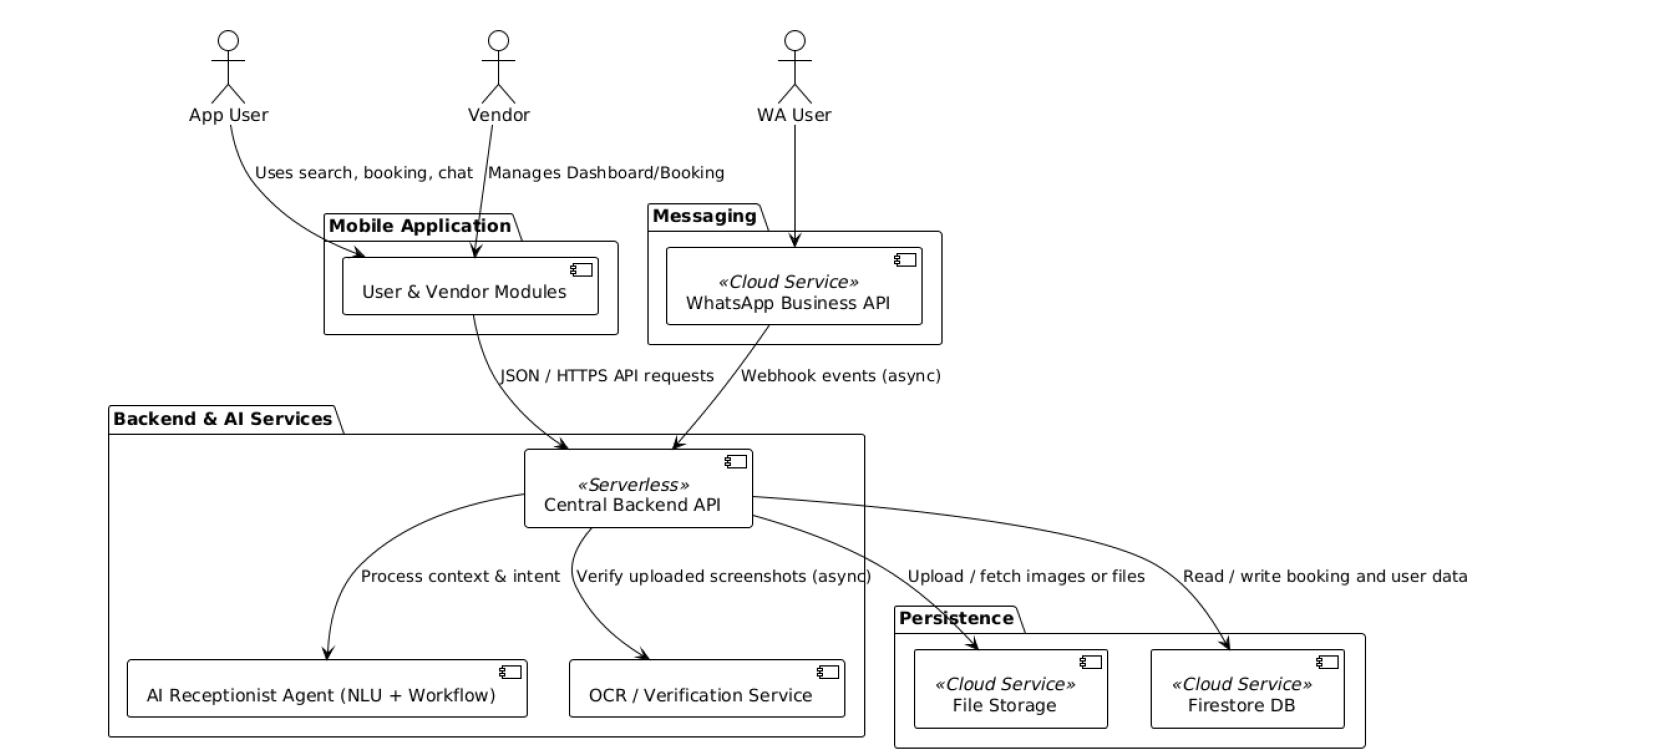
\includegraphics[width=0.95\textwidth]{images/system-overview.png}
  \caption{System block diagram for the BookForMe platform.}
  \label{fig:srs-block}
\end{figure}

\subsection{Component descriptions}
\begin{itemize}[leftmargin=1.2cm]
  \item \textbf{Customer mobile app} --- React Native (Expo). Handles discovery, booking, AI chat filter, and all social features. Communicates with the backend via HTTPS APIs.
  \item \textbf{Vendor dashboard} --- React Native. Profile management, live court calendar, pending payment review, and WhatsApp account linking.
  \item \textbf{Admin panel} --- React Native. Platform governance: vendor approval/moderation, slot generation, stale lock release, payment oversight.
  \item \textbf{AI agent backend} --- Python/FastAPI with LangGraph. Manages the WhatsApp webhook conversation loop, bilingual NLU via Groq, stateful booking workflow, and Firestore-backed concurrency control (OCC).
  \item \textbf{Cloud Firestore} --- Central NoSQL store for profiles, slots, bookings, conversation state, social data, and payment records.
  \item \textbf{WhatsApp Business API} --- Inbound webhooks and outbound messaging channel for the AI receptionist.
  \item \textbf{Firebase Authentication} --- Identity management for customers, vendors, and admins.
\end{itemize}

\section{System Screenshots}
\label{sec:srs-screenshots}

The following screenshots from the deployed BookForMe application illustrate the key user-facing and vendor-facing interfaces described in the functional requirements above.

\subsection{Authentication}

\begin{figure}[H]
  \centering
  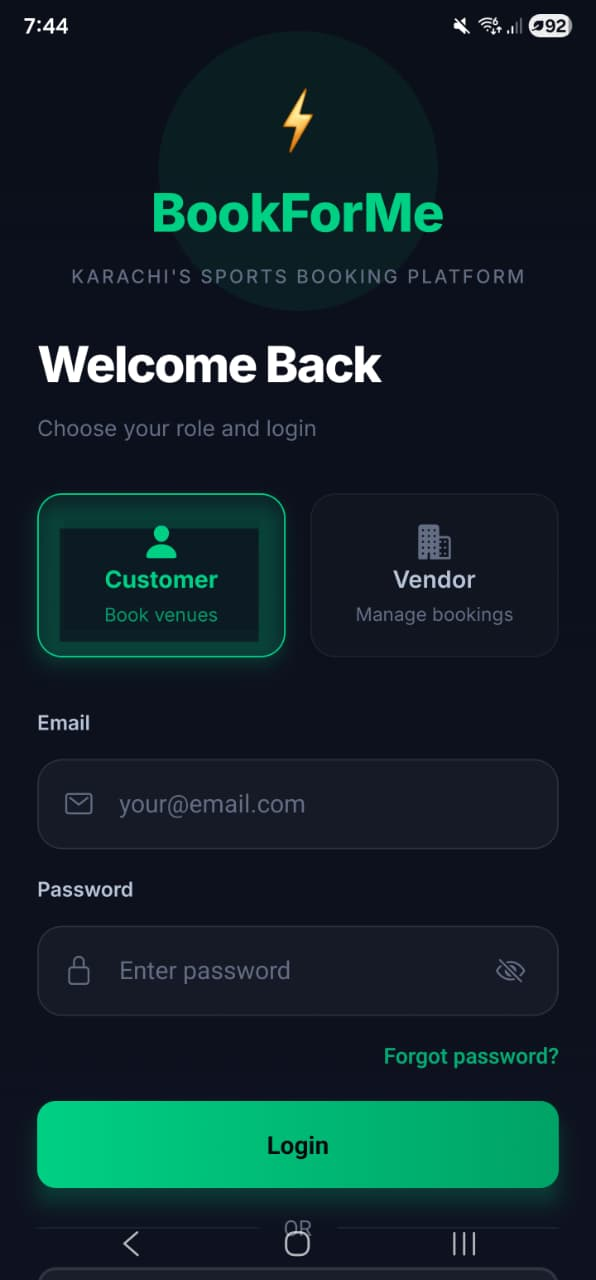
\includegraphics[width=0.45\textwidth]{images/Login.jpeg}
  \caption{Login screen with role selection (Customer or Vendor).}
  \label{fig:srs-login}
\end{figure}

\subsection{Customer application}

\begin{figure}[H]
  \centering
  \begin{minipage}[t]{0.45\textwidth}
    \centering
    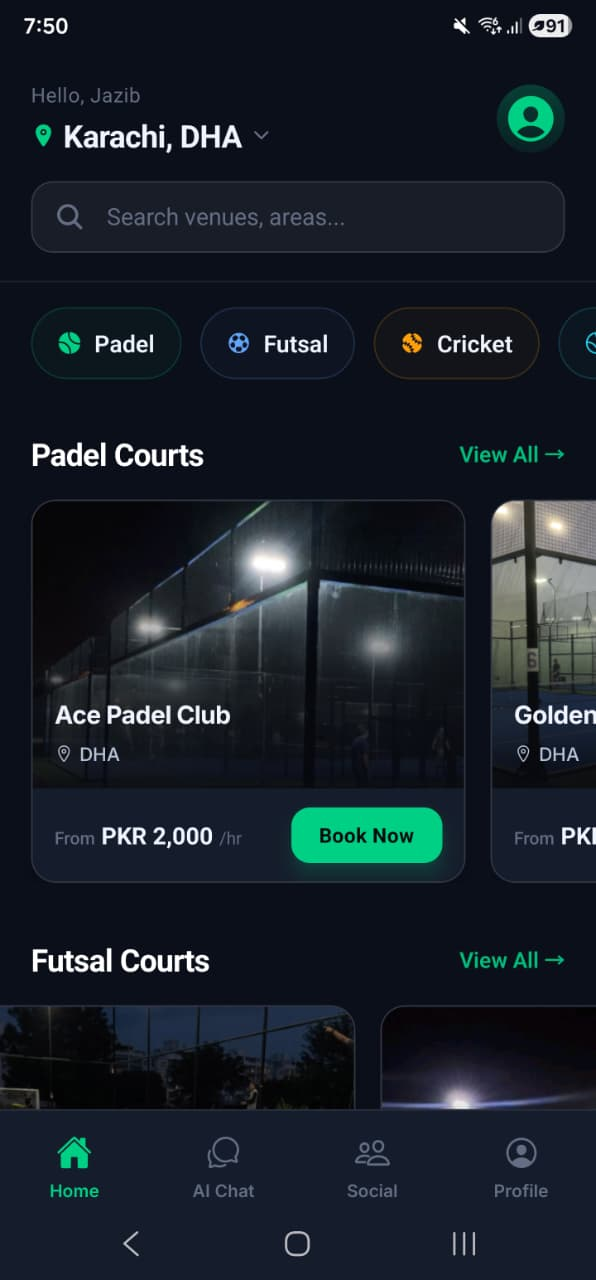
\includegraphics[width=\textwidth]{images/Home Page.jpeg}
    \caption{Customer home: venue discovery by sport and area.}
    \label{fig:srs-home}
  \end{minipage}
  \hfill
  \begin{minipage}[t]{0.45\textwidth}
    \centering
    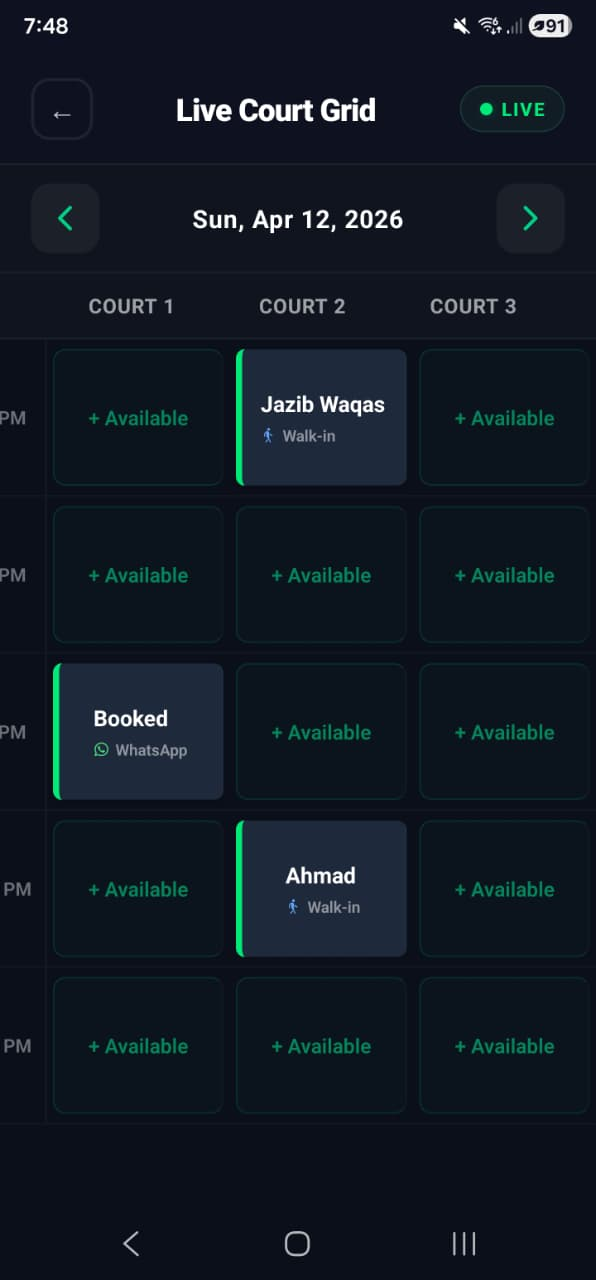
\includegraphics[width=\textwidth]{images/Booking slots.jpeg}
    \caption{Live court grid showing real-time slot availability and booking source.}
    \label{fig:srs-slots}
  \end{minipage}
\end{figure}

\begin{figure}[H]
  \centering
  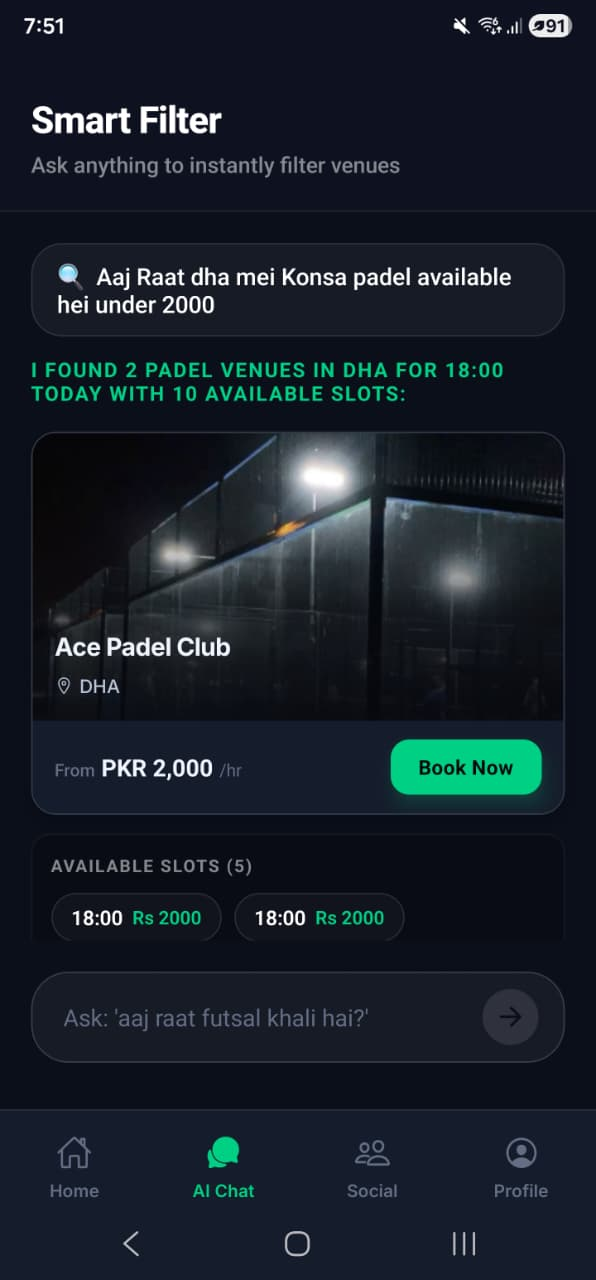
\includegraphics[width=0.45\textwidth]{images/AI chat App.jpeg}
  \caption{In-app smart filter: AI chat parses Roman Urdu/English queries and returns filtered venues with available slots.}
  \label{fig:srs-aichat}
\end{figure}

\subsection{Social hub}

\begin{figure}[H]
  \centering
  \begin{minipage}[t]{0.3\textwidth}
    \centering
    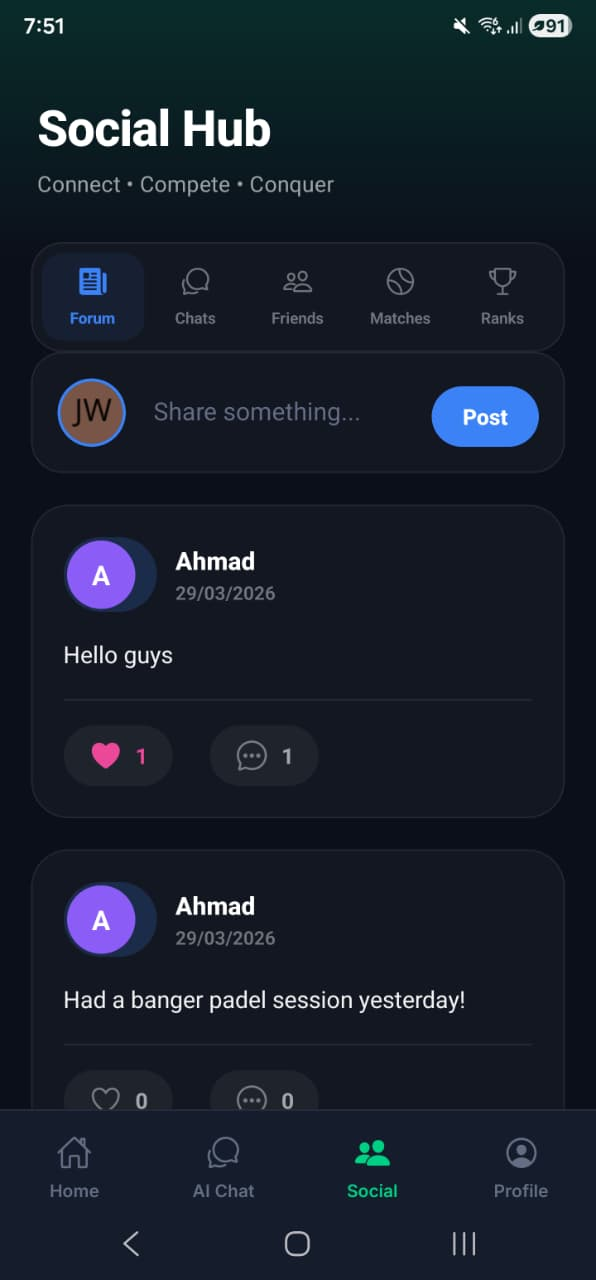
\includegraphics[width=\textwidth]{images/Forum.jpeg}
    \caption{Community forum.}
    \label{fig:srs-forum}
  \end{minipage}
  \hfill
  \begin{minipage}[t]{0.3\textwidth}
    \centering
    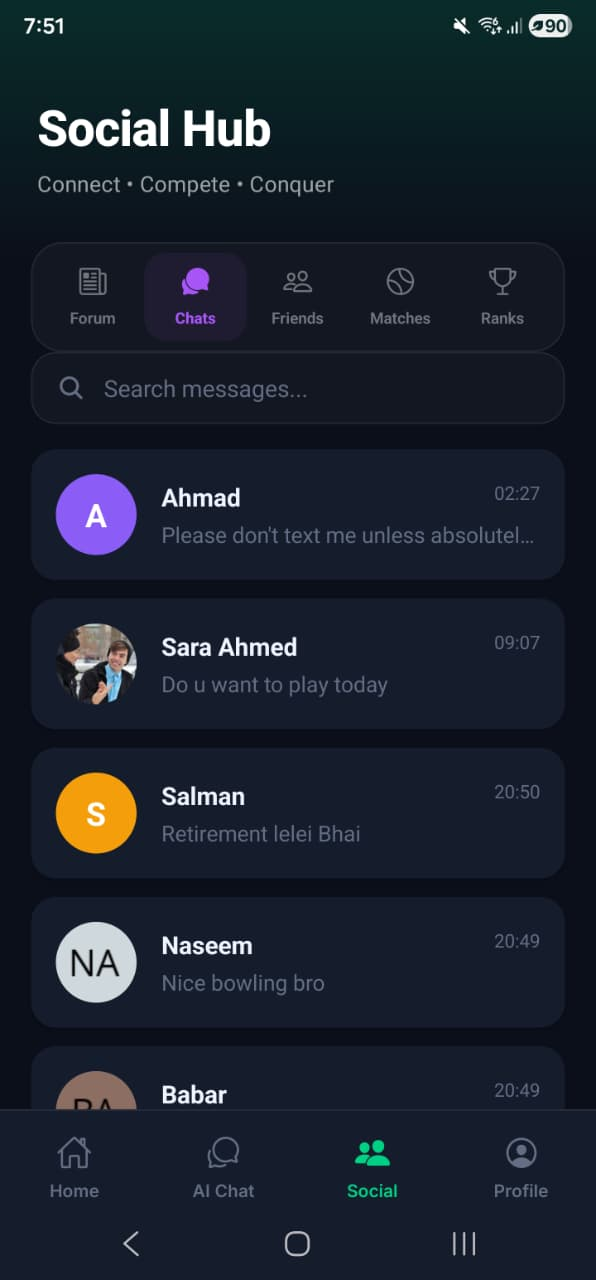
\includegraphics[width=\textwidth]{images/Chat Page.jpeg}
    \caption{Direct messages.}
    \label{fig:srs-chat}
  \end{minipage}
  \hfill
  \begin{minipage}[t]{0.3\textwidth}
    \centering
    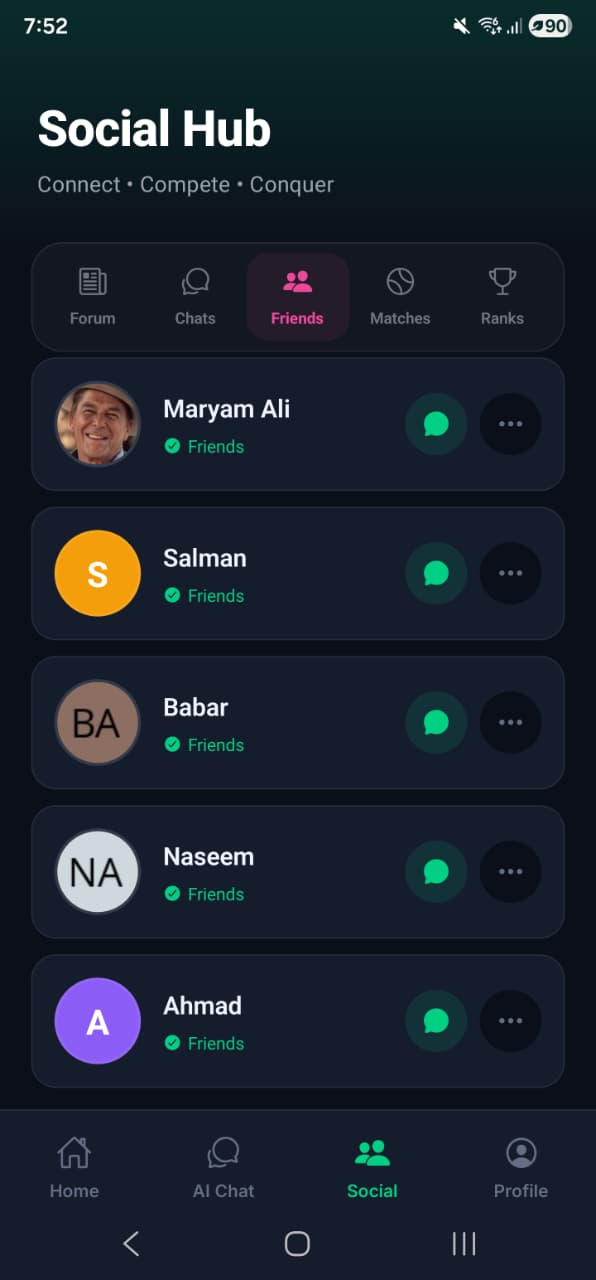
\includegraphics[width=\textwidth]{images/WhatsApp Image 2026-04-12 at 7.53.09 PM.jpeg}
    \caption{Friends list.}
    \label{fig:srs-friends}
  \end{minipage}
\end{figure}

\begin{figure}[H]
  \centering
  \begin{minipage}[t]{0.45\textwidth}
    \centering
    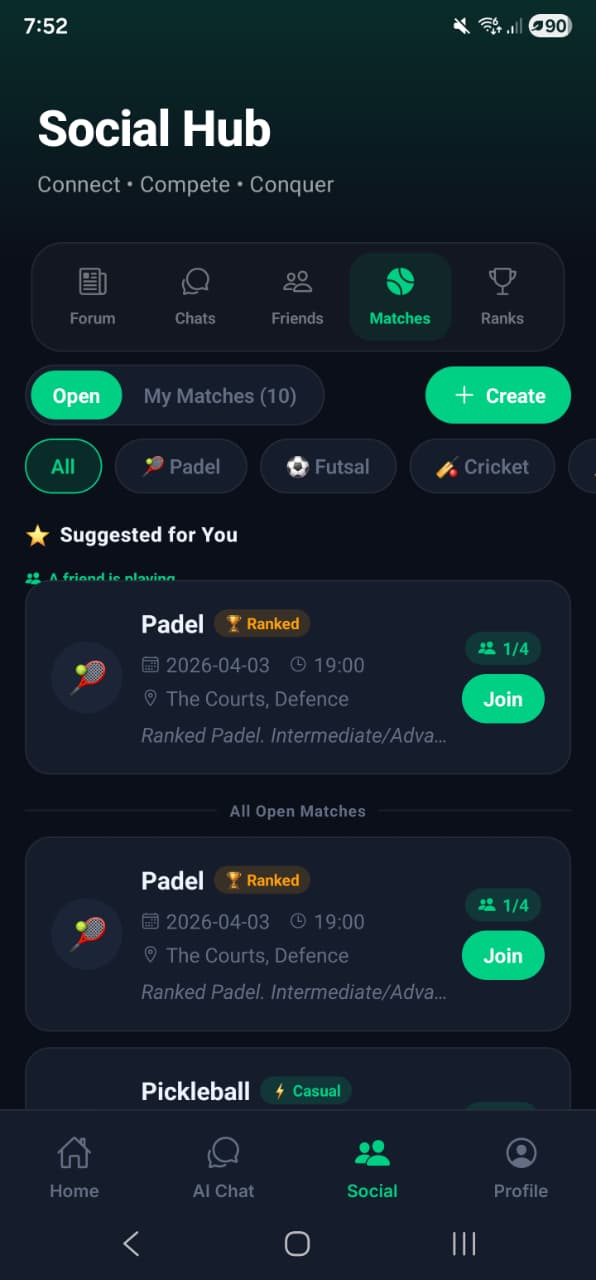
\includegraphics[width=\textwidth]{images/Match Page.jpeg}
    \caption{Open matches: casual and ranked lobbies.}
    \label{fig:srs-matches}
  \end{minipage}
  \hfill
  \begin{minipage}[t]{0.45\textwidth}
    \centering
    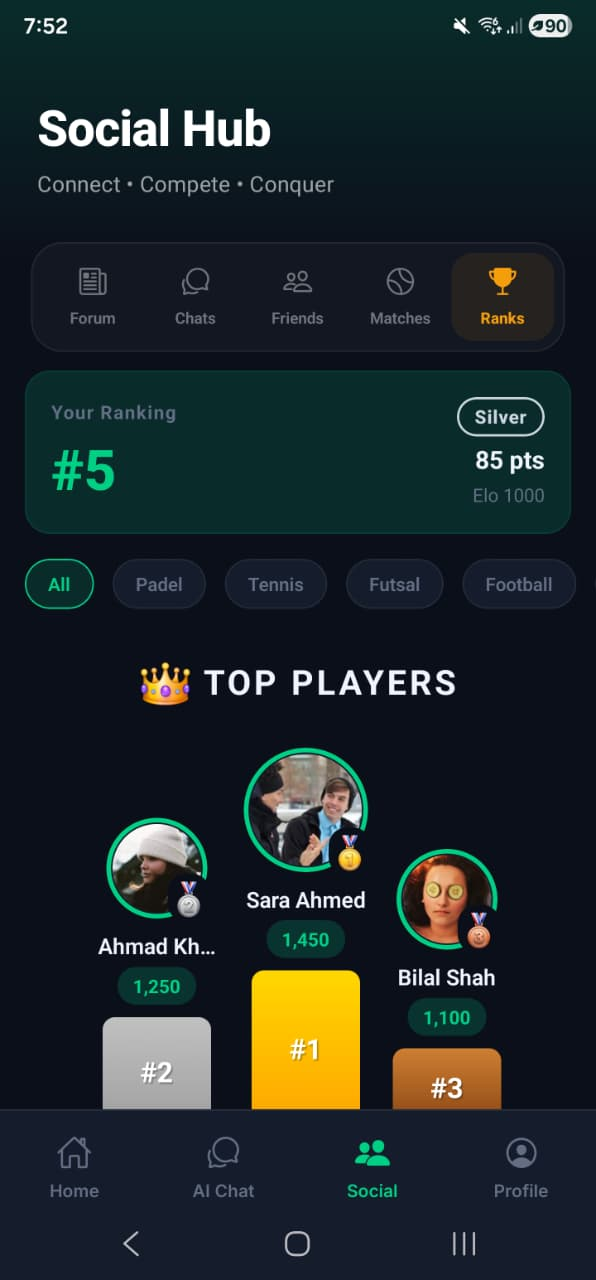
\includegraphics[width=\textwidth]{images/Leadboard.jpeg}
    \caption{Ranked leaderboard with Elo ratings and tiers.}
    \label{fig:srs-leaderboard}
  \end{minipage}
\end{figure}

\subsection{Vendor dashboard}

\begin{figure}[H]
  \centering
  \begin{minipage}[t]{0.45\textwidth}
    \centering
    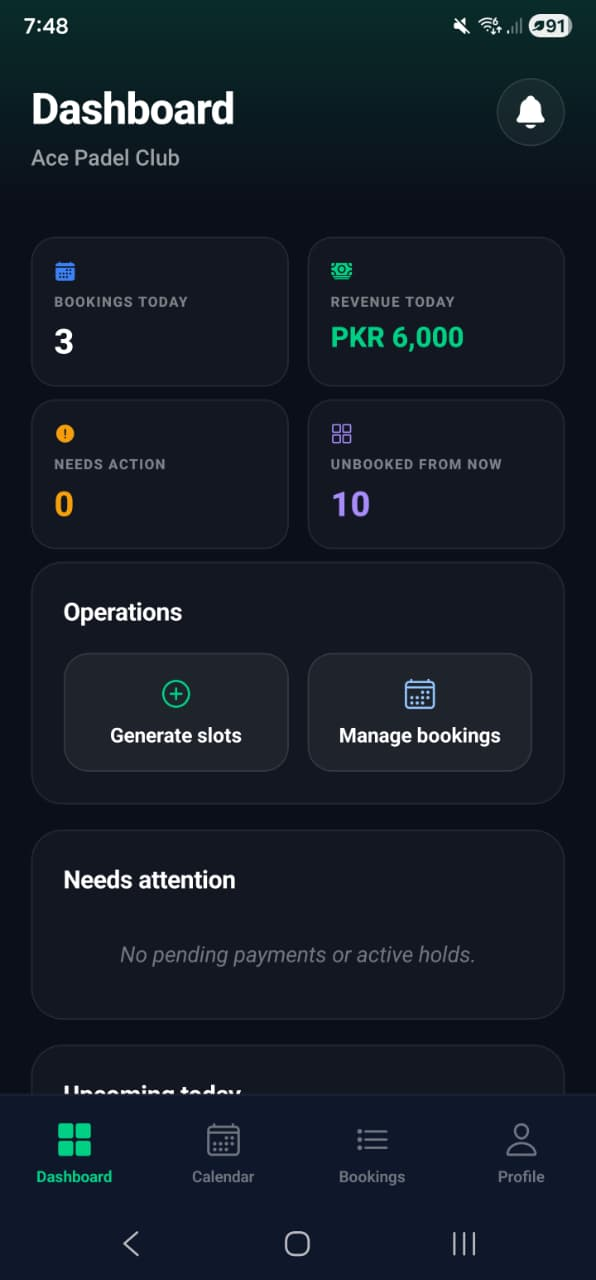
\includegraphics[width=\textwidth]{images/Vendor Dashboard.jpeg}
    \caption{Vendor dashboard: daily stats, pending actions, slot operations, and upcoming bookings.}
    \label{fig:srs-vendor}
  \end{minipage}
  \hfill
  \begin{minipage}[t]{0.45\textwidth}
    \centering
    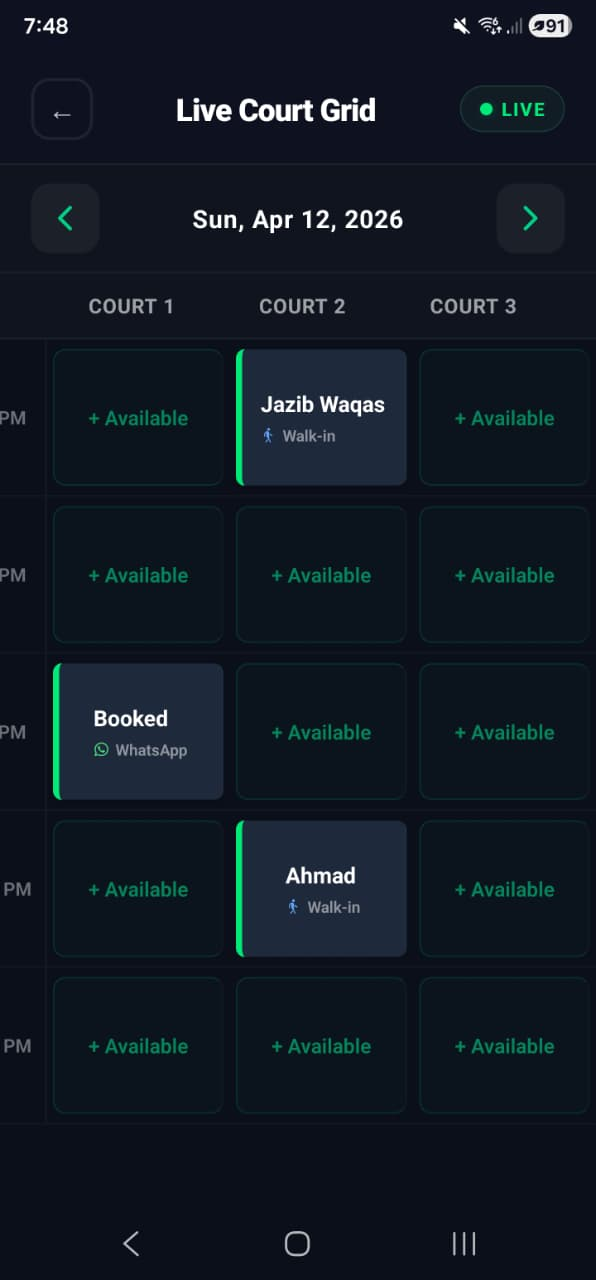
\includegraphics[width=\textwidth]{images/Booking slots.jpeg}
    \caption{Live court grid calendar: per-court slot status with WhatsApp and walk-in booking sources.}
    \label{fig:srs-vendor-calendar}
  \end{minipage}
\end{figure}

\subsection{AI receptionist (WhatsApp)}

\begin{figure}[H]
  \centering
  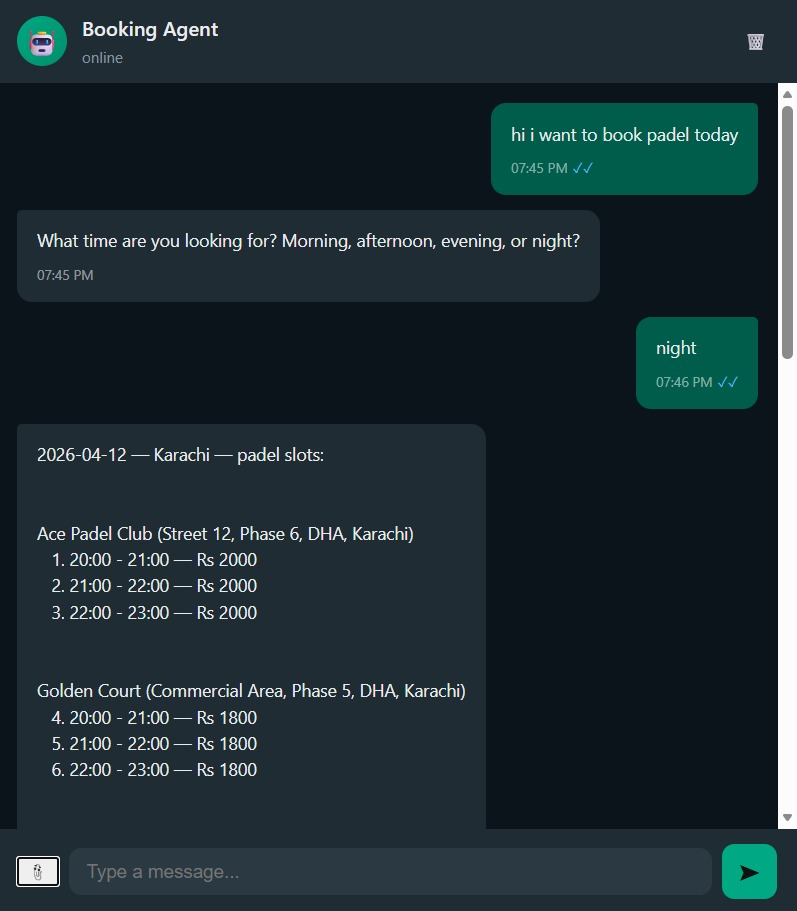
\includegraphics[width=0.75\textwidth]{images/WhatsApp Converstation.jpeg}
  \caption{WhatsApp AI receptionist: bilingual booking conversation returning available padel slots across multiple venues.}
  \label{fig:srs-whatsapp}
\end{figure}

\subsection{Admin control panel}

\begin{figure}[H]
  \centering
  \begin{minipage}[t]{0.45\textwidth}
    \centering
    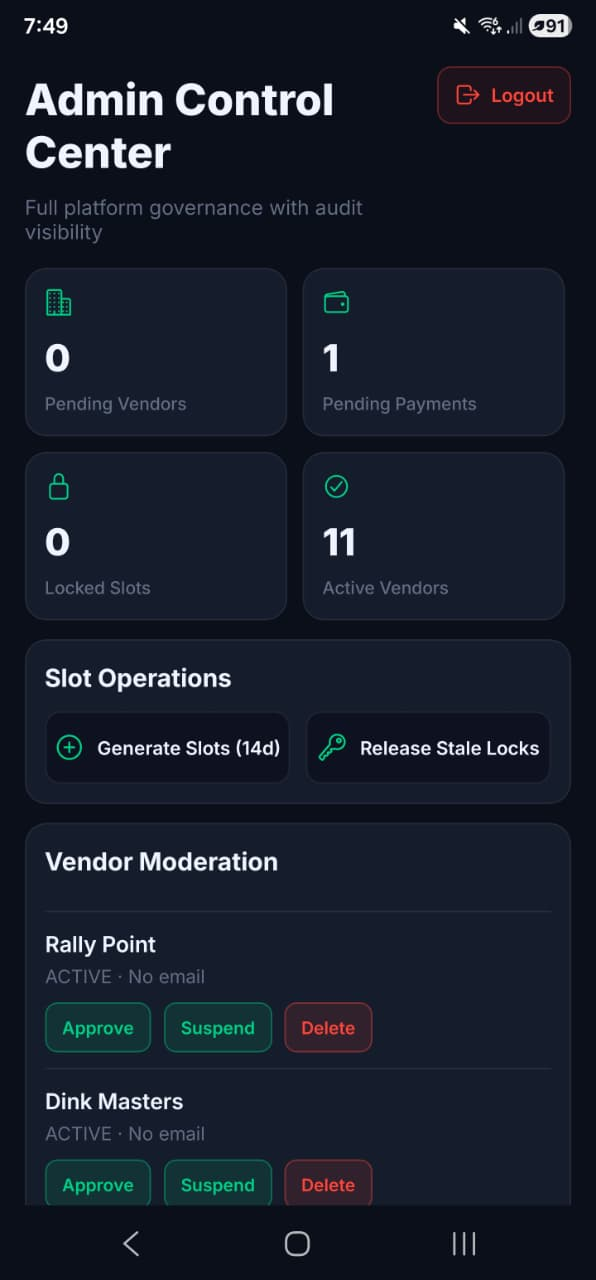
\includegraphics[width=\textwidth]{images/Admin Dashboard.jpeg}
    \caption{Admin control center: platform-wide stats, slot generation, and vendor moderation.}
    \label{fig:srs-admin1}
  \end{minipage}
  \hfill
  \begin{minipage}[t]{0.45\textwidth}
    \centering
    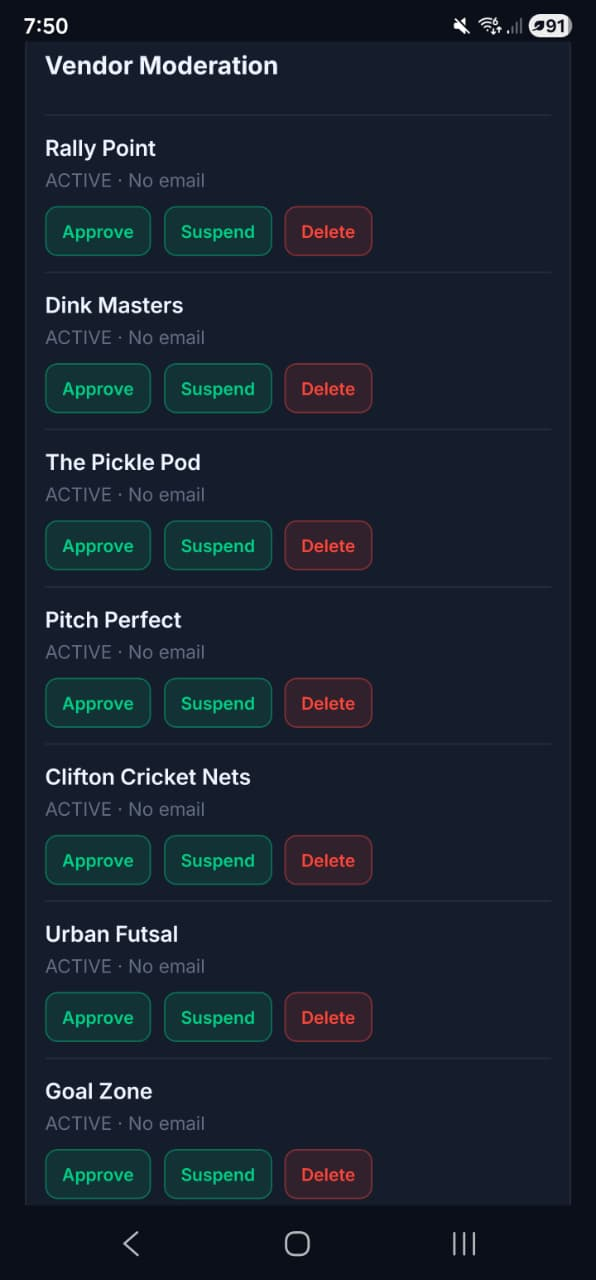
\includegraphics[width=\textwidth]{images/Admin Dashboard (2).jpeg}
    \caption{Admin vendor moderation: approve, suspend, or delete registered vendors.}
    \label{fig:srs-admin2}
  \end{minipage}
\end{figure}
